% =============================================================================
% ICLR 2027 COLLABORATIVE MANUSCRIPT
% =============================================================================
% Overleaf setup:
%   1. Upload this file together with iclr2027_conference.sty,
%      iclr2027_conference.bst, and OVERLEAF_ICLR2027_REFERENCES.bib.
%   2. Set this file as the Overleaf Main document.
%   3. Keep \iclrfinalcopy commented for anonymous submission.
%
% Collaboration workflow:
%   - Visible draft annotations are ON by default.
%   - Before any submission build, switch \showcommentstrue to
%     \showcommentsfalse and search the source for TODO, CHECK, and CLAIM.
%   - Source comments beginning with CLAIM STATUS record the evidence ceiling.
%   - Do not add results without a seed-level record and a frozen metric label.
%
% CLAIM STATUS (current):
%   [EXACT]      One-sided stop-gradient decomposition and factorial identities.
%   [FORMAL]     Seeds 3--5, q=256, 256 kimg factorial and 256--1024 curves.
%   [SECONDARY]  Seeds 14--18 learning-curve sensitivity analysis.
%   [SUPPORTING] Frozen-state RAdam virtual-update diagnostics.
%   [PENDING]    Prospectively unseen cohort, AUC/time-to-quality primary test,
%                budget-resolved target-component audit, second weighting rule.
% =============================================================================

\documentclass{article}
\usepackage{iclr2027_conference,times}

\usepackage{amsmath,amssymb,mathtools,bm}
\usepackage{booktabs}
\usepackage{graphicx}
\usepackage{xcolor}
\usepackage{hyperref}
\usepackage{url}

% -----------------------------------------------------------------------------
% Collaboration annotations. These must be disabled for submission.
% -----------------------------------------------------------------------------
\newif\ifshowcomments
\showcommentstrue
% \showcommentsfalse

\definecolor{todored}{RGB}{180,35,35}
\definecolor{theoryblue}{RGB}{25,85,160}
\definecolor{empiricalgreen}{RGB}{20,120,80}
\definecolor{claimpurple}{RGB}{110,55,145}

\newcommand{\todo}[1]{%
  \ifshowcomments{\color{todored}\textbf{[TODO: #1]}}\fi}
\newcommand{\theorynote}[1]{%
  \ifshowcomments{\color{theoryblue}\textbf{[THEORY CHECK: #1]}}\fi}
\newcommand{\empnote}[1]{%
  \ifshowcomments{\color{empiricalgreen}\textbf{[EMPIRICAL CHECK: #1]}}\fi}
\newcommand{\claimnote}[1]{%
  \ifshowcomments{\color{claimpurple}\textbf{[CLAIM CEILING: #1]}}\fi}

\newcommand{\sg}{\operatorname{sg}}
\newcommand{\Dsg}{\mathcal{D}^{\mathrm{sg}}_\theta}
\newcommand{\Ropt}{R_{\mathrm{opt}}}

\title{The Optimization Geometry of Consistency Gaps}

% Authors are hidden by the ICLR style while \iclrfinalcopy is commented.
\author{Anonymous Authors}

% \iclrfinalcopy % Uncomment only for the accepted camera-ready version.

\begin{document}

\maketitle

\begin{abstract}
Consistency training pairs states separated by a temporal gap, yet the
optimization meaning of changing this gap is unclear. We show that an ECT gap
change is a composite intervention that exactly decomposes into a detached
target-endpoint change and an explicit loss-rescaling change. These components
factorize at the instantaneous objective-gradient level under the one-sided
stop-gradient training derivative. They need not factorize after separately
trained models enter different parameter trajectories. In a controlled
target-by-denominator experiment, the complete enlarged-gap intervention
improves the 256-kimg NFE1 FID in all three formal training seeds, while the
denominator contrasts and factorial interaction are not directionally stable.
Budget-resolved evaluation from 256 to 1024 kimg shows large early quality
differences followed by smaller, seed-dependent contrasts and changing arm
rankings. A five-seed secondary cohort likewise selects different arms at 1024
kimg under NFE1 and NFE2. These results position consistency gaps primarily as
controls of finite-budget learning trajectories and time-to-quality, rather
than as hyperparameters that define a universally superior final model.
\end{abstract}

\todo{Abstract: re-check wording after the prospectively unseen cohort is
complete; do not replace the current evidence status before unblinding.}

\section{Introduction}
\label{sec:introduction}

Consistency models support one- or few-step generation by learning a mapping
that is consistent along a noise trajectory \citep{song2023consistency}.
Easy Consistency Tuning (ECT) constructs paired states at different times and
trains an online prediction against a detached target
\citep{geng2024consistency}. The temporal separation between those states---the
\emph{consistency gap}---is therefore a basic design choice. A larger gap can
substantially change early FID and KID even when different legal gap schedules
can identify the same ideal consistency mapping under strong assumptions.

This creates the central puzzle of the paper:
\emph{why can changing the consistency gap alter finite-budget learning speed
and generation quality when the ideal mapping may be unchanged?}
The answer is not that a gap is merely a different discretization step. In the
ECT objective studied here, changing the gap simultaneously changes the
detached target endpoint and the explicit denominator applied to the loss.
These interventions are exactly separable at one fixed model state, but
separate training runs feed their gradients into different parameter and
optimizer trajectories. Objective-level identities therefore constrain the
instantaneous intervention without determining finite-training outcomes.

Our contributions are:
\begin{enumerate}
  \item \textbf{Exact objective decomposition.}
  We define the one-sided stop-gradient training derivative and derive an exact,
  finite-gap decomposition into target-endpoint and denominator-rescaling
  components. We also derive exact identities for a four-cell
  target-by-denominator factorial.

  \item \textbf{Controlled finite-training disentanglement.}
  We train the four factorial arms from matched initial conditions. At the
  formal 256-kimg NFE1 endpoint, target-related contrasts favor the enlarged
  endpoint in all three seeds, whereas denominator and interaction contrasts
  vary in direction. The design does not license a percentage decomposition of
  quality.

  \item \textbf{Learning-trajectory evidence.}
  Across seven budgets from 256 to 1024 kimg, early arm differences contract
  and rankings become dependent on seed and sampling NFE. A separate five-seed
  secondary analysis shows the same absence of a universal long-budget winner.
\end{enumerate}

\paragraph{Scope relative to optimizer mechanisms.}
Stateful adaptive optimization provides one reason why an instantaneous
gradient identity need not become an update or endpoint identity. We use
frozen-state RAdam diagnostics only to support this boundary. We do not claim
that optimizer memory causes the observed FID differences or mediates a fixed
percentage of the gap effect.

\claimnote{The paper's novelty is the ECT composite intervention and its
finite-training geometry. Do not re-center the narrative on RAdam history,
balanced beta, optimizer scale invariance, or a universal best gap.}

\section{Consistency gaps as composite interventions}
\label{sec:theory}

\subsection{Ideal target and endpoint-invariance intuition}
\label{sec:theory-ideal-endpoint}

Let $x_t$ denote a state on a coupled trajectory and let
$\mathcal{T}_{t\rightarrow r}$ transport that state from $t$ to $r\leq t$.
We call a gap schedule $S$ \emph{legal} on a support $\mathcal{X}$ if every
supported time $t$ is connected to a common anchor $t_\star$ by a finite chain
$t=t_0>t_1>\cdots>t_m=t_\star$ of scheduled edges. Suppose that:
\begin{enumerate}
  \item the transport is exact and compositional,
  $\mathcal{T}_{r\rightarrow s}\!\circ\mathcal{T}_{t\rightarrow r}
  =\mathcal{T}_{t\rightarrow s}$;
  \item all scheduled edges are covered by the population objective;
  \item the function class can attain zero consistency residual on those edges;
  \item optimization reaches such a population solution; and
  \item the mapping is fixed at the common anchor by
  $F(x,t_\star)=b(x)$.
\end{enumerate}
Then zero residual along the schedule telescopes to
\begin{equation}
  F^\star(x_t,t)
  =F^\star\!\left(\mathcal{T}_{t\rightarrow t_1}(x_t),t_1\right)
  =\cdots
  =b\!\left(\mathcal{T}_{t\rightarrow t_\star}(x_t)\right).
  \label{eq:ideal-endpoint-invariance}
\end{equation}
Consequently, any two legal schedules that share the same transport, support,
and anchor identify the same ideal consistency mapping on their reachable
support. The gap schedule can change the constraints presented during training
without changing the ideal endpoint mapping under these assumptions.

Equation~\eqref{eq:ideal-endpoint-invariance} is an ideal identification
statement. Without a common anchor, connectivity, population support coverage,
an attainable zero-residual solution, or successful population optimization,
schedule invariance need not hold. It is not a claim about finite-capacity,
finite-data, or incompletely optimized models.

\theorynote{Keep the endpoint-invariance statement conditional. If the method
notation later replaces exact transport by a numerical solver, revise the
transport assumption rather than weakening it silently.}

\subsection{Exact ECT composite intervention}
\label{sec:theory-composite-intervention}

The preceding ideal invariance does not make the ECT training intervention
scalar. For one coupled ECT sample, let
$x_t=y+t\varepsilon$, $x_r=y+r\varepsilon$, $\Delta=t-r>0$, and define
\begin{equation}
  D_t=f_\theta(x_t,t),\qquad
  T_r=\sg\!\left[f_\theta(x_r,r)\right],\qquad
  e_r=D_t-T_r,\qquad
  \phi(e)=\lVert e\rVert_2 .
  \label{eq:ect-residual}
\end{equation}
Here $\sg$ preserves the target's forward value but suppresses its parameter
derivative. Formally, introduce a two-parameter lifted loss
$\widetilde\ell(\theta,\bar\theta)$. The one-sided stop-gradient training
derivative is
\begin{equation}
  \Dsg\ell
  :=\left.
  \partial_\theta\widetilde\ell(\theta,\bar\theta)
  \right|_{\bar\theta=\theta}.
  \label{eq:sg-training-derivative}
\end{equation}
This is not the ordinary derivative along the parameter diagonal, which would
also differentiate the target copy. For $e_r\neq0$, the ECT objective and its
one-sided training derivative are
\begin{equation}
  \ell(r,\Delta)=\frac{\phi(e_r)}{\Delta},
  \qquad
  g(r,\Delta):=\Dsg\ell(r,\Delta)
  =\frac{1}{\Delta}J_t^\top u_r,
  \qquad
  J_t:=\partial_\theta D_t,
  \quad
  u_r:=\frac{e_r}{\lVert e_r\rVert_2}.
  \label{eq:exact-ect-gradient}
\end{equation}

Consider a baseline gap $\Delta_1$ with target
$r_1=t-\Delta_1$ and a probe gap $\Delta_g$ with target
$r_g=t-\Delta_g$, evaluated at the same parameter value and with the same
online realization. Setting $s:=\Delta_1/\Delta_g$, direct substitution gives
the exact finite-gap decompositions
\begin{align}
  \ell_g
  &=s\ell_1
    +\underbrace{\frac{\phi(e_{r_g})-\phi(e_{r_1})}{\Delta_g}}
      _{\tau^{(\ell)}_{\mathrm{tar}}},
  \label{eq:exact-ect-loss-decomposition}\\
  g_g
  &=s g_1
    +\underbrace{\frac{1}{\Delta_g}J_t^\top
      \left(u_{r_g}-u_{r_1}\right)}
      _{\tau^{(g)}_{\mathrm{tar}}}.
  \label{eq:exact-ect-gradient-decomposition}
\end{align}
We call $s\ell_1$ and $s g_1$ the \emph{denominator-rescaling component}, and
$\tau^{(\ell)}_{\mathrm{tar}}$ and $\tau^{(g)}_{\mathrm{tar}}$ the
\emph{target-endpoint component}. Their joint change is the
\emph{ECT composite gap intervention}.
Equations~\eqref{eq:exact-ect-loss-decomposition}--
\eqref{eq:exact-ect-gradient-decomposition} require neither a small-gap
approximation nor an optimizer model. Only the denominator-rescaling component
is exactly scalar. The total training derivative is scalar-equivalent to the
baseline only when its target-endpoint component vanishes or happens to align
with the baseline derivative.

\subsection{Exact factorial identities}
\label{sec:theory-factorial-identities}

The composite intervention yields an exact objective-gradient factorialization.
For a matched sample, define the four cells
\begin{equation}
  A=(r_1,\Delta_1),\qquad
  B=(r_g,\Delta_g),\qquad
  C=(r_g,\Delta_1),\qquad
  D=(r_1,\Delta_g),
  \label{eq:factorial-cells}
\end{equation}
where the first coordinate selects the detached target endpoint and the second
selects the explicit denominator. Because the denominator multiplies the
objective and its one-sided training derivative externally,
\begin{align}
  \ell_B&=s\ell_C,&
  \ell_D&=s\ell_A,&
  \ell_B-\ell_D&=s(\ell_C-\ell_A),
  \label{eq:factorial-loss-identities}\\
  g_B&=s g_C,&
  g_D&=s g_A,&
  g_B-g_D&=s(g_C-g_A).
  \label{eq:factorial-gradient-identities}
\end{align}
The corresponding factorial interactions obey
\begin{equation}
  I_\ell:=\ell_B-\ell_C-\ell_D+\ell_A
  =(s-1)(\ell_C-\ell_A),
  \qquad
  I_g:=g_B-g_C-g_D+g_A
  =(s-1)(g_C-g_A).
  \label{eq:exact-factorial-interactions}
\end{equation}
For an unclipped global gap multiplier, $s=1/g$ is common to all samples and
the identities also hold after minibatch aggregation. With clipping, they
remain exact per sample but generally do not reduce to one batch-wide scalar.

\emph{These identities factorize the intervention at the objective-gradient
level; they do not imply an additive or seed-invariant factorization of
finite-training quality.}
Once the four arms follow separate parameter trajectories, the matched
quantities in Eqs.~\eqref{eq:factorial-loss-identities}--
\eqref{eq:exact-factorial-interactions} are no longer held fixed. The theory
therefore motivates the factorial experiment without predetermining its
finite-training quality contrasts.

\section{Formal target-by-denominator experiment}
\label{sec:factorial-experiment}

\subsection{Design and estimands}

We evaluate the decomposition with a $2\times2$ intervention in the q=256
ECT setting. The enlarged-gap condition uses a global multiplier $g=1.10$.
The four arms are shown in Table~\ref{tab:arms}. Arms share the same starting
checkpoint, data order, sampled times, noise, dropout stream, optimizer,
learning rate, EMA, and numerical settings; only the target endpoint and
explicit denominator assignment differ.

\begin{table}[t]
  \caption{Target-by-denominator factorial. The labels baseline and enlarged
  denote the endpoint or denominator induced by the corresponding gap rule.}
  \label{tab:arms}
  \centering
  \begin{tabular}{cll}
    \toprule
    Arm & Detached target endpoint & Explicit denominator \\
    \midrule
    A & baseline & baseline \\
    B & enlarged & enlarged \\
    C & enlarged & baseline \\
    D & baseline & enlarged \\
    \bottomrule
  \end{tabular}
\end{table}

The formal factorial uses training seeds 3--5. The prespecified primary
endpoint is NFE1 FID-50k at 256 kimg; KID-50k and NFE2 are separate readouts.
Each contrast is first formed within a training seed. Training seed---not
budget, NFE, or metric---is the independent unit. Negative FID or KID
contrasts favor the first named arm.

\empnote{Methods owner: add the final architecture, batch size, optimizer
hyperparameters, EMA, data preprocessing, and hardware table from the frozen
run manifests. Do not infer missing values from memory.}

\subsection{Early finite-training contrasts}

At 256 kimg and NFE1, the complete intervention $B-A$, the target-only
contrast $C-A$, and the target contrast within the enlarged denominator
$B-D$ are favorable in all three seeds for both FID and KID
(Table~\ref{tab:factorial-256}). The denominator-only contrast $D-A$ and the
factorial interaction vary in direction. These observations are consistent
with a substantial early role for the target endpoint. They neither establish
that the denominator is irrelevant nor identify an additive percentage of the
quality change.

\begin{table}[t]
  \caption{Formal 256-kimg NFE1 seed-level factorial contrasts. Values are
  means over three paired training-seed contrasts; the negative-seed columns
  report the number of seeds with a negative contrast.}
  \label{tab:factorial-256}
  \centering
  \small
  \begin{tabular}{lrrrr}
    \toprule
    Contrast & Mean FID & Negative seeds & Mean KID & Negative seeds \\
    \midrule
    $B-A$ & $-11.5408$ & $3/3$ & $-0.016225$ & $3/3$ \\
    $C-A$ & $ -9.8676$ & $3/3$ & $-0.007294$ & $3/3$ \\
    $B-D$ & $-14.3405$ & $3/3$ & $-0.021344$ & $3/3$ \\
    $D-A$ & $ +2.7997$ & $2/3$ & $+0.005119$ & $1/3$ \\
    $B-C-D+A$ & $-4.4729$ & $2/3$ & $-0.014049$ & $2/3$ \\
    \bottomrule
  \end{tabular}
\end{table}

NFE2 does not supply a uniform replication of the NFE1 factorial pattern.
Its seed-level contrasts are more heterogeneous, which motivates treating
sampling NFE as a distinct readout rather than an additional replicate.

\claimnote{Describe the target result as directionally consistent at this
endpoint. Do not write \emph{target geometry explains X percent},
\emph{denominator does not matter}, or
\emph{the factorial endpoint validates the algebra}.}

\section{Gap components reshape learning trajectories}
\label{sec:learning-trajectories}

\subsection{Formal budget-resolved curves}

We evaluate all four arms at
$K\in\{256,384,512,640,768,896,1024\}$ kimg for seeds 3--5, NFE1 and NFE2.
The resulting matrix contains 168 completed FID/KID-50k evaluation jobs
($3$ seeds $\times4$ arms $\times7$ budgets $\times2$ NFE values). All formal
jobs passed the recorded artifact and status audit.

Figure~\ref{fig:seed-resolved-curves} shows every formal seed, arm, budget, and
NFE readout. Table~\ref{tab:ba-curve} reports the NFE1 FID contrast for the
complete intervention. The separation is large at 256--384 kimg and much
smaller from 512 kimg onward. From 512 kimg, only two of three seeds favor $B$,
and the cohort-mean contrast changes sign at 512 kimg. At NFE2, the mean $B-A$
FID contrast likewise changes from $-48.0770$ at 256 kimg and $-28.8781$ at
384 kimg to $-0.0377$ at 1024 kimg, with seed heterogeneity at later budgets.
The evidence therefore supports a transient learning-trajectory effect more
directly than a stable endpoint ordering.

\begin{figure}[t]
  \centering
  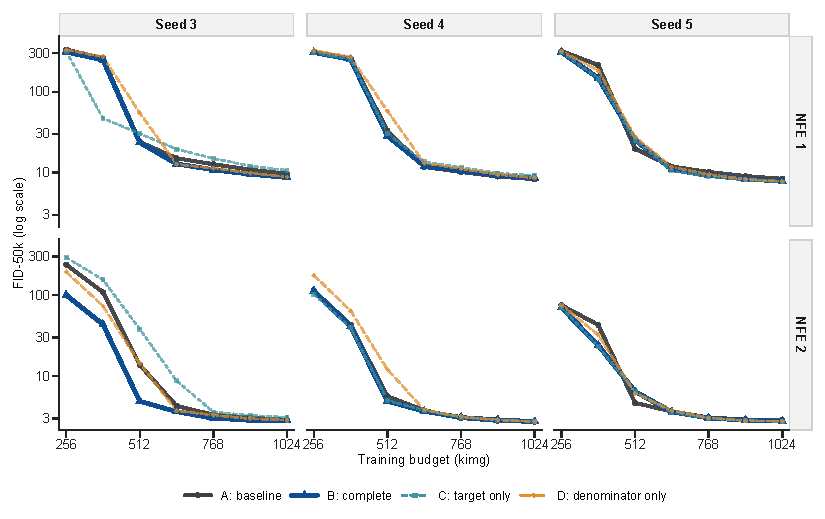
\includegraphics[width=\linewidth]
    {figures/figure2_seed_resolved_learning_curves.pdf}
  \caption{\textbf{Seed-resolved finite-budget learning trajectories.}
  Columns show formal training seeds 3--5 and rows show NFE1 and NFE2.
  Each curve contains the seven frozen budgets from 256 to 1024 kimg; every
  point is a FID-50k evaluation. Arms A and B are emphasized, while the
  target-only arm C and denominator-only arm D provide factorial context.
  The logarithmic FID axis exposes both the large early separations and the
  later contraction and crossings. Training seed is the independent unit;
  budgets and NFE readouts are repeated measurements, not additional
  replicates.}
  \label{fig:seed-resolved-curves}
\end{figure}

\begin{table}[t]
  \caption{Budget-resolved NFE1 FID contrast for the complete intervention in
  formal seeds 3--5. Negative values favor arm B.}
  \label{tab:ba-curve}
  \centering
  \small
  \begin{tabular}{rrr}
    \toprule
    Budget (kimg) & Mean $B-A$ FID & Seeds favoring B \\
    \midrule
     256 & $-11.5408$ & $3/3$ \\
     384 & $-28.9498$ & $3/3$ \\
     512 & $ +0.2762$ & $2/3$ \\
     640 & $ -0.9574$ & $2/3$ \\
     768 & $ -0.8300$ & $2/3$ \\
     896 & $ -0.5755$ & $2/3$ \\
    1024 & $ -0.4502$ & $2/3$ \\
    \bottomrule
  \end{tabular}
\end{table}

The component contrasts themselves are also budget dependent
(Figure~\ref{fig:factorial-contrast-curves}). Target, denominator, and
interaction trajectories can change sign even when their 256-kimg summaries
are directionally clear. This is the quality-level distinction between an
exact matched-state factorial identity and a factorial comparison after
separate training.

\begin{figure}[t]
  \centering
  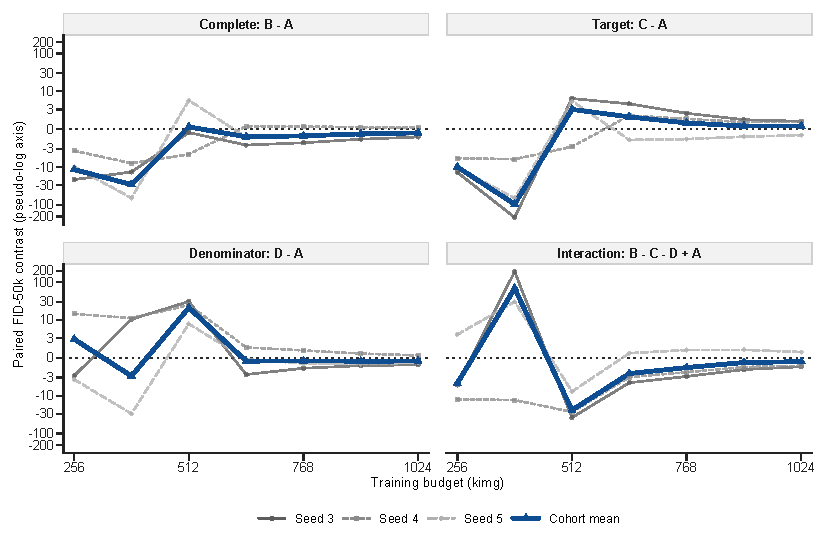
\includegraphics[width=\linewidth]
    {figures/figure4_budget_dependent_factorial_contrasts.pdf}
  \caption{\textbf{Budget-dependent NFE1 factorial contrasts.}
  Panels show the paired FID-50k contrasts $B-A$, $C-A$, $D-A$, and
  $B-C-D+A$ for each formal training seed and their descriptive cohort mean.
  Negative values favor the first named arm. The shared signed pseudo-log axis
  is linear near zero ($\sigma=1$) and logarithmic in both tails, allowing
  early large contrasts and later near-zero variation to remain visible on the
  same scale. The dotted line marks zero. All three seed trajectories are
  displayed; the blue mean is not treated as an additional replicate.}
  \label{fig:factorial-contrast-curves}
\end{figure}

\subsection{Secondary long-budget sensitivity}

Seeds 14--18 provide a post-preregistration secondary sensitivity analysis.
They comprise 20 complete trajectories, six budgets from 384 to 1024 kimg, and
240 completed FID/KID-50k evaluation jobs. Early NFE1 cohort means remain
widely separated: at 384 kimg the FID means for A/B/C/D are
$252.07/170.84/222.62/161.19$, whereas at 640 kimg they are
$14.17/14.43/13.27/14.98$. By 1024 kimg, arm D has the lowest NFE1 cohort-mean
FID and KID, while arm A has the lowest NFE2 cohort-mean FID and KID
(Table~\ref{tab:secondary-1024}).

\begin{table}[t]
  \caption{Secondary seeds 14--18 at 1024 kimg. Entries are five-seed cohort
  means and are sensitivity summaries, not additional formal replicates.}
  \label{tab:secondary-1024}
  \centering
  \small
  \begin{tabular}{crrrr}
    \toprule
    & \multicolumn{2}{c}{NFE1} & \multicolumn{2}{c}{NFE2} \\
    \cmidrule(lr){2-3}\cmidrule(lr){4-5}
    Arm & FID & KID & FID & KID \\
    \midrule
    A & 9.1761 & 0.005563 & \textbf{2.8768} & \textbf{0.001006} \\
    B & 8.9022 & 0.005506 & 2.9201 & 0.001114 \\
    C & 9.1882 & 0.005696 & 2.9472 & 0.001099 \\
    D & \textbf{8.6604} & \textbf{0.005362} & 2.8898 & 0.001025 \\
    \bottomrule
  \end{tabular}
\end{table}

The secondary cohort does not convert one arm into a universal recommendation.
Instead, it shows that the long-budget ordering depends on the realized
training trajectory and the sampler readout. Together with the formal curves,
the result shifts the empirical question from
\emph{which gap wins at one checkpoint?} to
\emph{how does the intervention change the budget required to reach a given
quality?}

\empnote{Figure 3: predefine log-FID AUC and time-to-quality only for the new
prospectively frozen cohort. Existing curves can illustrate these quantities
but must not be retroactively labeled confirmatory.}

\section{Why instantaneous identities do not determine trajectories}
\label{sec:stateful-trajectories}

The exact identities in Section~\ref{sec:theory} hold at one parameter value
and for matched stochastic inputs. Training composes such local derivatives
through parameter-dependent targets, changing Jacobians, stochastic gradients,
and optimizer state. Even an exactly scalar current-gradient intervention need
not produce a scalar next update under a stateful adaptive optimizer whose
moments were accumulated along a different history.

We use a frozen-state RAdam factorial only to demonstrate this possibility.
Let
\begin{equation}
  \Ropt(U_1,U_0)
  :=\frac{\lVert U_1-c^\star U_0\rVert_2}{\lVert U_0\rVert_2},
  \qquad
  c^\star:=\frac{\langle U_1,U_0\rangle}{\lVert U_0\rVert_2^2},
  \label{eq:optimizer-residual}
\end{equation}
measure the residual after best scalar alignment of two virtual updates.
Across seeds 3--5, the seed medians are $0.074$--$0.088$ for observed
gradients with real accumulated state, $0.467$--$0.491$ with reset state,
$0.049$--$0.077$ for an exact-scalar gradient under real state, and
$0.0006$--$0.0017$ when both the gradient and state are reduced to the
fresh scalar control. Thus the realized gradient residual and accumulated
state interact at the next-update level.

A separately frozen moment-transport proposal failed its held-out preflight:
all 12 rows increased rather than decreased the registered divergence, so no
continuation training or FID/KID evaluation was launched. This is a useful
stop signal. The optimizer diagnostics support the statement that
objective-gradient identities do not automatically survive stateful
optimization; they do not identify the cause of the finite-training quality
differences.

\claimnote{Keep this section compact. PR65 is a next-update diagnostic and
PR66 is a NO-GO result. Neither is endpoint mechanism closure.}

\section{Discussion, generalization, and limitations}
\label{sec:discussion}

\paragraph{Objective factorization versus outcome factorization.}
The exact target-by-denominator identities are strongest when interpreted
locally: they specify what changes in one matched ECT objective and training
derivative. The factorial training experiment asks a different question:
what happens after those components generate separate trajectories? The
observed budget, seed, and NFE dependence is not a failure of the algebra; it
is the finite-training phenomenon that the algebra isolates.

\paragraph{Learning efficiency is the prospective target.}
The present curves motivate a primary estimand based on NFE1 log-FID
learning-curve area over fixed budgets, with time-to-FID thresholds as
secondary summaries. These estimands require a prospectively frozen, unseen
training-seed cohort. Existing seeds are used to establish and motivate the
trajectory hypothesis, not to claim held-out confirmation of a retrospectively
chosen AUC.

\paragraph{General weighting rules.}
The ECT setting above uses an explicit $1/\Delta$ denominator. For a general
weight $w(t,r)$, the same one-sided derivative gives
\begin{equation}
  g_g
  =\frac{w_g}{w_1}g_1
   +w_gJ_t^\top\left(u_{r_g}-u_{r_1}\right).
  \label{eq:general-weight-decomposition}
\end{equation}
This suggests a direct generalization test: compare the realized scalar
component under the CIFAR-style gap-dependent weighting with a
gap-independent weighting regime. Equation~\eqref{eq:general-weight-decomposition}
is an algebraic extension; a second-regime network audit and training result
remain pending.

\paragraph{Current limitations.}
The formal budget-resolved evidence contains three independent training seeds
in one CIFAR-10 ECT setting, complemented by five post-preregistration
secondary seeds. FID and KID share an Inception-based representation, and NFE1
and NFE2 produce different rankings. The current evidence therefore supports
trajectory-dependent learning effects in this setting, not a universal
statement over architectures, datasets, weighting rules, or samplers.
A prospectively unseen cohort, a budget-resolved target-gradient audit, and a
second weighting regime are the highest-value extensions.

\todo{Related-work owner: complete the citation audit for consistency
training, weighting schedules, finite-budget optimization, and adaptive
optimizer scale effects. Preserve the bounded novelty statement.}

\section{Conclusion}
\label{sec:conclusion}

A consistency-gap change in ECT is an exact composite intervention: it changes
both the detached target endpoint and the explicit loss denominator. Those
components factorize at the instantaneous objective-gradient level, but the
factorization does not determine quality after separate finite-training
trajectories emerge. Controlled four-arm experiments show large early
differences, later contraction, and rankings that vary with seed and sampling
NFE. The practical role of a consistency gap is therefore best understood as
reshaping learning trajectories and time-to-quality, not as defining a
universally superior endpoint.

\subsection*{AI use statement}

Generative AI tools were used to assist with manuscript organization, LaTeX
formatting, prose editing, and consistency checking of author-provided
mathematical derivations and experimental records. They were not used to
generate experimental measurements or to replace author verification of
mathematical claims. The authors reviewed AI-assisted text, equations, and
numerical transcriptions against the repository records and take responsibility
for the final content.

\todo{All authors must review this required ICLR 2027 disclosure and add any
other reportable AI uses before submission.}

\subsection*{Ethics statement}

This work studies optimization behavior on a standard public image benchmark
and introduces no human-participant study or private dataset. The main risks
are scientific: overgeneralizing from a limited set of seeds or presenting
secondary analyses as confirmatory. We address these risks by reporting the
training seed as the independent unit, separating formal and secondary cohorts,
and preserving the stated claim ceilings.

\subsection*{Reproducibility statement}

The supplementary material records the four-arm intervention, seed and budget
matrix, frozen evaluation protocol, artifact-completeness audits, and the
assumptions behind the exact decomposition. The code and machine-readable
records will be provided through an anonymous supplementary artifact for
review.

\todo{Create and verify the anonymous artifact URL; do not link an
identity-revealing repository in the double-blind submission.}

\bibliography{OVERLEAF_ICLR2027_REFERENCES}
\bibliographystyle{iclr2027_conference}

\appendix

\section{Proof of ideal endpoint invariance}
\label{app:ideal-proof}

Fix a supported $(x_t,t)$ and let
$t=t_0>t_1>\cdots>t_m=t_\star$ be a scheduled chain. Zero population residual
on edge $(t_j,t_{j+1})$ gives
\begin{equation}
  F^\star(x_{t_j},t_j)
  =F^\star(\mathcal{T}_{t_j\rightarrow t_{j+1}}(x_{t_j}),t_{j+1}).
\end{equation}
Applying this equality successively and using compositional transport yields
\begin{equation}
  F^\star(x_t,t)
  =F^\star(\mathcal{T}_{t\rightarrow t_\star}(x_t),t_\star).
\end{equation}
The common anchor condition then gives
$F^\star(x_t,t)=b(\mathcal{T}_{t\rightarrow t_\star}(x_t))$.
The right-hand side depends on the transport and anchor, not on the particular
legal chain. Hence any two legal schedules satisfying the assumptions identify
the same mapping on their common reachable support.

\section{Evaluation and artifact audit summary}
\label{app:evaluation-audit}

\begin{table}[h]
  \caption{Status of the evidence used in the main text. A completed job means
  that the recorded evaluation and its required artifacts passed the
  corresponding repository audit.}
  \label{tab:evidence-status}
  \centering
  \small
  \begin{tabular}{p{0.25\linewidth}p{0.18\linewidth}p{0.44\linewidth}}
    \toprule
    Evidence block & Status & Scope \\
    \midrule
    Formal factorial & Complete &
    Seeds 3--5; four arms; 256 kimg; NFE1/2; 24 FID/KID-50k cells. \\
    Formal learning curves & Complete &
    Seeds 3--5; four arms; seven budgets; NFE1/2; 168 FID/KID-50k jobs. \\
    Secondary curves & Complete, secondary &
    Seeds 14--18; four arms; six budgets; NFE1/2; 240 FID/KID-50k jobs. \\
    RAdam virtual updates & Supporting only &
    Frozen-state next-update geometry; no endpoint causal claim. \\
    Moment transport & Scientific NO-GO &
    Held-out preflight worsened all 12 rows; no continuation training. \\
    Prospective cohort & Pending &
    Unseen seeds, frozen log-FID AUC, contraction, and time-to-quality. \\
    \bottomrule
  \end{tabular}
\end{table}

\section{Collaboration checklist}
\label{app:collaboration-checklist}

% This checklist is deliberately visible while comments are enabled.
\begin{enumerate}
  \item \todo{Replace the methods placeholder with values copied from frozen
  manifests and obtain a second-author verification.}
  \item \todo{Build seed-resolved learning-curve and budget-dependent
  factorial-contrast figures; preserve training seed as the unit.}
  \item \todo{Freeze the prospective cohort and primary AUC before launching
  any new training run.}
  \item \todo{Complete the target-component audit without using it as a
  mediation claim.}
  \item \todo{Run the literature and citation audit, including exact overlap
  boundaries for adaptive-optimizer scale effects.}
  \item \todo{Disable comments, resolve every TODO/CHECK/CLAIM marker, compile
  with the official ICLR 2027 style, and confirm the 9-page main-text limit.}
\end{enumerate}

\end{document}
